\documentclass[twoside]{book}

% Packages required by doxygen
\usepackage{fixltx2e}
\usepackage{calc}
\usepackage{doxygen}
\usepackage[export]{adjustbox} % also loads graphicx
\usepackage{graphicx}
\usepackage[utf8]{inputenc}
\usepackage{makeidx}
\usepackage{multicol}
\usepackage{multirow}
\PassOptionsToPackage{warn}{textcomp}
\usepackage{textcomp}
\usepackage[nointegrals]{wasysym}
\usepackage[table]{xcolor}

% Font selection
\usepackage[T1]{fontenc}
\usepackage[scaled=.90]{helvet}
\usepackage{courier}
\usepackage{amssymb}
\usepackage{sectsty}
\renewcommand{\familydefault}{\sfdefault}
\allsectionsfont{%
  \fontseries{bc}\selectfont%
  \color{darkgray}%
}
\renewcommand{\DoxyLabelFont}{%
  \fontseries{bc}\selectfont%
  \color{darkgray}%
}
\newcommand{\+}{\discretionary{\mbox{\scriptsize$\hookleftarrow$}}{}{}}

% Page & text layout
\usepackage{geometry}
\geometry{%
  a4paper,%
  top=2.5cm,%
  bottom=2.5cm,%
  left=2.5cm,%
  right=2.5cm%
}
\tolerance=750
\hfuzz=15pt
\hbadness=750
\setlength{\emergencystretch}{15pt}
\setlength{\parindent}{0cm}
\setlength{\parskip}{3ex plus 2ex minus 2ex}
\makeatletter
\renewcommand{\paragraph}{%
  \@startsection{paragraph}{4}{0ex}{-1.0ex}{1.0ex}{%
    \normalfont\normalsize\bfseries\SS@parafont%
  }%
}
\renewcommand{\subparagraph}{%
  \@startsection{subparagraph}{5}{0ex}{-1.0ex}{1.0ex}{%
    \normalfont\normalsize\bfseries\SS@subparafont%
  }%
}
\makeatother

% Headers & footers
\usepackage{fancyhdr}
\pagestyle{fancyplain}
\fancyhead[LE]{\fancyplain{}{\bfseries\thepage}}
\fancyhead[CE]{\fancyplain{}{}}
\fancyhead[RE]{\fancyplain{}{\bfseries\leftmark}}
\fancyhead[LO]{\fancyplain{}{\bfseries\rightmark}}
\fancyhead[CO]{\fancyplain{}{}}
\fancyhead[RO]{\fancyplain{}{\bfseries\thepage}}
\fancyfoot[LE]{\fancyplain{}{}}
\fancyfoot[CE]{\fancyplain{}{}}
\fancyfoot[RE]{\fancyplain{}{\bfseries\scriptsize Generated by Doxygen }}
\fancyfoot[LO]{\fancyplain{}{\bfseries\scriptsize Generated by Doxygen }}
\fancyfoot[CO]{\fancyplain{}{}}
\fancyfoot[RO]{\fancyplain{}{}}
\renewcommand{\footrulewidth}{0.4pt}
\renewcommand{\chaptermark}[1]{%
  \markboth{#1}{}%
}
\renewcommand{\sectionmark}[1]{%
  \markright{\thesection\ #1}%
}

% Indices & bibliography
\usepackage{natbib}
\usepackage[titles]{tocloft}
\setcounter{tocdepth}{3}
\setcounter{secnumdepth}{5}
\makeindex

% Hyperlinks (required, but should be loaded last)
\usepackage{ifpdf}
\ifpdf
  \usepackage[pdftex,pagebackref=true]{hyperref}
\else
  \usepackage[ps2pdf,pagebackref=true]{hyperref}
\fi
\hypersetup{%
  colorlinks=true,%
  linkcolor=blue,%
  citecolor=blue,%
  unicode%
}

% Custom commands
\newcommand{\clearemptydoublepage}{%
  \newpage{\pagestyle{empty}\cleardoublepage}%
}

\usepackage{caption}
\captionsetup{labelsep=space,justification=centering,font={bf},singlelinecheck=off,skip=4pt,position=top}

%===== C O N T E N T S =====

\begin{document}

% Titlepage & ToC
\hypersetup{pageanchor=false,
             bookmarksnumbered=true,
             pdfencoding=unicode
            }
\pagenumbering{alph}
\begin{titlepage}
\vspace*{7cm}
\begin{center}%
{\Large My Project }\\
\vspace*{1cm}
{\large Generated by Doxygen 1.8.12}\\
\end{center}
\end{titlepage}
\clearemptydoublepage
\pagenumbering{roman}
\tableofcontents
\clearemptydoublepage
\pagenumbering{arabic}
\hypersetup{pageanchor=true}

%--- Begin generated contents ---
\chapter{Hierarchical Index}
\section{Class Hierarchy}
This inheritance list is sorted roughly, but not completely, alphabetically\+:\begin{DoxyCompactList}
\item \contentsline{section}{Myob\+File\+Controller}{\pageref{class_myob_file_controller}}{}
\item \contentsline{section}{M\+Y\+O\+Bto\+A\+T\+Ocontroller}{\pageref{class_m_y_o_bto_a_t_ocontroller}}{}
\item Q\+Dialog\begin{DoxyCompactList}
\item \contentsline{section}{Myob\+Output\+Dialog}{\pageref{class_myob_output_dialog}}{}
\item \contentsline{section}{M\+Y\+O\+Bto\+A\+T\+O\+Main\+Dialog}{\pageref{class_m_y_o_bto_a_t_o_main_dialog}}{}
\end{DoxyCompactList}
\item Q\+Main\+Window\begin{DoxyCompactList}
\item \contentsline{section}{A\+T\+Oassignment\+Main\+Window}{\pageref{class_a_t_oassignment_main_window}}{}
\end{DoxyCompactList}
\end{DoxyCompactList}

\chapter{Class Index}
\section{Class List}
Here are the classes, structs, unions and interfaces with brief descriptions\+:\begin{DoxyCompactList}
\item\contentsline{section}{\hyperlink{class_a_t_oassignment_main_window}{A\+T\+Oassignment\+Main\+Window} \\*Main window }{\pageref{class_a_t_oassignment_main_window}}{}
\item\contentsline{section}{\hyperlink{class_myob_file_controller}{Myob\+File\+Controller} }{\pageref{class_myob_file_controller}}{}
\item\contentsline{section}{\hyperlink{class_myob_output_dialog}{Myob\+Output\+Dialog} }{\pageref{class_myob_output_dialog}}{}
\item\contentsline{section}{\hyperlink{class_m_y_o_bto_a_t_ocontroller}{M\+Y\+O\+Bto\+A\+T\+Ocontroller} }{\pageref{class_m_y_o_bto_a_t_ocontroller}}{}
\item\contentsline{section}{\hyperlink{class_m_y_o_bto_a_t_o_main_dialog}{M\+Y\+O\+Bto\+A\+T\+O\+Main\+Dialog} }{\pageref{class_m_y_o_bto_a_t_o_main_dialog}}{}
\end{DoxyCompactList}

\chapter{Class Documentation}
\hypertarget{class_a_t_oassignment_main_window}{}\section{A\+T\+Oassignment\+Main\+Window Class Reference}
\label{class_a_t_oassignment_main_window}\index{A\+T\+Oassignment\+Main\+Window@{A\+T\+Oassignment\+Main\+Window}}


Main window.  




{\ttfamily \#include $<$atoassignmentmainwindow.\+h$>$}

Inheritance diagram for A\+T\+Oassignment\+Main\+Window\+:\begin{figure}[H]
\begin{center}
\leavevmode
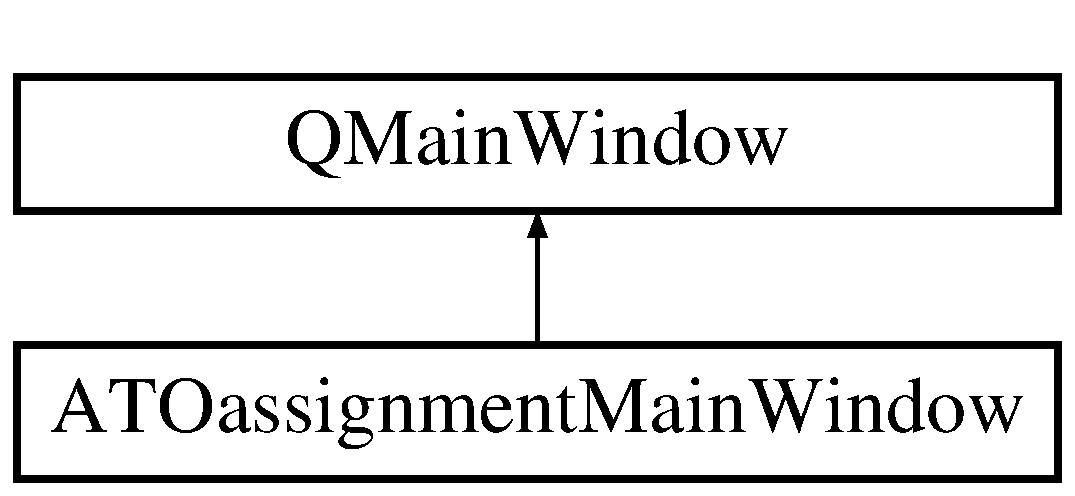
\includegraphics[height=2.000000cm]{class_a_t_oassignment_main_window}
\end{center}
\end{figure}
\subsection*{Public Member Functions}
\begin{DoxyCompactItemize}
\item 
\hypertarget{class_a_t_oassignment_main_window_a443871b5a99b1725e128b0c4186ac66d}{}\label{class_a_t_oassignment_main_window_a443871b5a99b1725e128b0c4186ac66d} 
{\bfseries A\+T\+Oassignment\+Main\+Window} (Q\+Widget $\ast$parent=0)
\end{DoxyCompactItemize}


\subsection{Detailed Description}
Main window. 

Class creates window on start of program and get user to click button to start 

The documentation for this class was generated from the following files\+:\begin{DoxyCompactItemize}
\item 
A\+T\+Oassignment/atoassignmentmainwindow.\+h\item 
A\+T\+Oassignment/atoassignmentmainwindow.\+cpp\end{DoxyCompactItemize}

\hypertarget{class_myob_file_controller}{}\section{Myob\+File\+Controller Class Reference}
\label{class_myob_file_controller}\index{Myob\+File\+Controller@{Myob\+File\+Controller}}


{\ttfamily \#include $<$myobfilecontroller.\+h$>$}

\subsection*{Public Member Functions}
\begin{DoxyCompactItemize}
\item 
\hypertarget{class_myob_file_controller_a931398570ccda783b8b1add583fe28b7}{}\label{class_myob_file_controller_a931398570ccda783b8b1add583fe28b7} 
ifstream $\ast$ {\bfseries Open\+Myob\+File} ()
\item 
\hypertarget{class_myob_file_controller_a41b5275e6e58bf5a8c5bc2b02fad84c6}{}\label{class_myob_file_controller_a41b5275e6e58bf5a8c5bc2b02fad84c6} 
void {\bfseries set\+Parent\+Ptr} (Q\+Widget $\ast$parent)
\end{DoxyCompactItemize}


\subsection{Detailed Description}
Class creates pointer to ifstream object to open Myob file 

The documentation for this class was generated from the following files\+:\begin{DoxyCompactItemize}
\item 
A\+T\+Oassignment/myobfilecontroller.\+h\item 
A\+T\+Oassignment/myobfilecontroller.\+cpp\end{DoxyCompactItemize}

\hypertarget{class_myob_output_dialog}{}\section{Myob\+Output\+Dialog Class Reference}
\label{class_myob_output_dialog}\index{Myob\+Output\+Dialog@{Myob\+Output\+Dialog}}


{\ttfamily \#include $<$myoboutputdialog.\+h$>$}

Inheritance diagram for Myob\+Output\+Dialog\+:\begin{figure}[H]
\begin{center}
\leavevmode
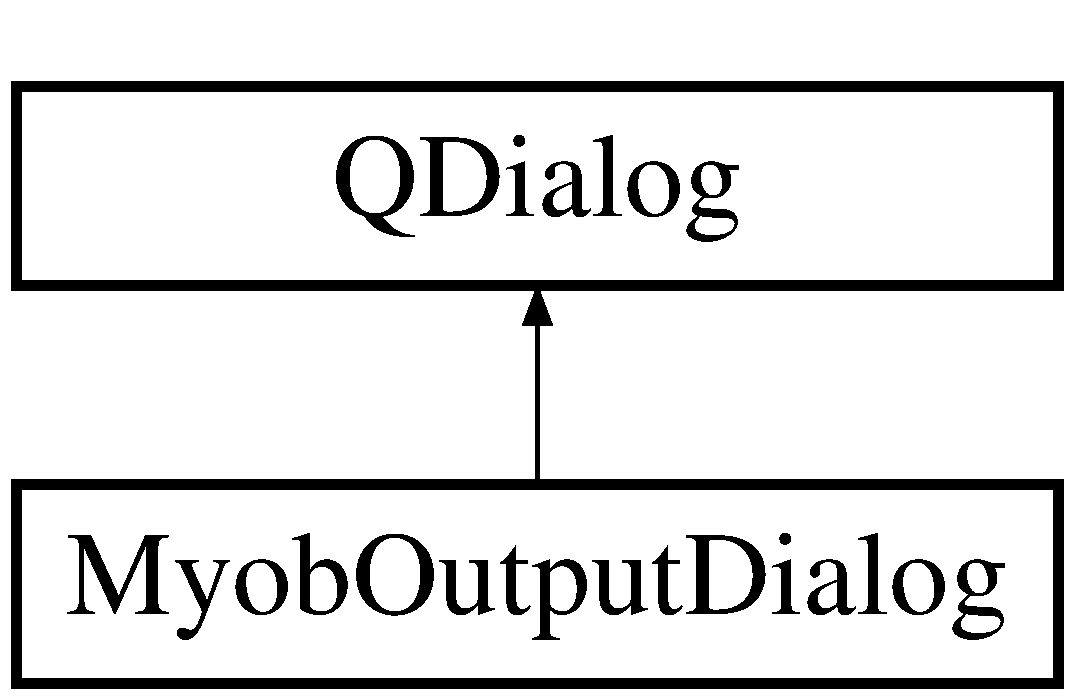
\includegraphics[height=2.000000cm]{class_myob_output_dialog}
\end{center}
\end{figure}
\subsection*{Public Member Functions}
\begin{DoxyCompactItemize}
\item 
\hypertarget{class_myob_output_dialog_a3307f232864fc026f8613103d2d1c315}{}\label{class_myob_output_dialog_a3307f232864fc026f8613103d2d1c315} 
{\bfseries Myob\+Output\+Dialog} (Q\+Widget $\ast$parent=0)
\item 
\hypertarget{class_myob_output_dialog_a85ab59f127e9365f1abf16fd2e64007b}{}\label{class_myob_output_dialog_a85ab59f127e9365f1abf16fd2e64007b} 
void {\bfseries set\+File\+Ptr} (ifstream $\ast$fileptr)
\item 
\hypertarget{class_myob_output_dialog_a7cbc13e0ae61980a6b491034b85825ac}{}\label{class_myob_output_dialog_a7cbc13e0ae61980a6b491034b85825ac} 
void {\bfseries display\+Text} ()
\end{DoxyCompactItemize}


\subsection{Detailed Description}
Class creates window to display Myob output which opens from M\+Y\+OB to A\+TO main main dialog window 

The documentation for this class was generated from the following files\+:\begin{DoxyCompactItemize}
\item 
A\+T\+Oassignment/myoboutputdialog.\+h\item 
A\+T\+Oassignment/myoboutputdialog.\+cpp\end{DoxyCompactItemize}

\hypertarget{class_m_y_o_bto_a_t_ocontroller}{}\section{M\+Y\+O\+Bto\+A\+T\+Ocontroller Class Reference}
\label{class_m_y_o_bto_a_t_ocontroller}\index{M\+Y\+O\+Bto\+A\+T\+Ocontroller@{M\+Y\+O\+Bto\+A\+T\+Ocontroller}}


{\ttfamily \#include $<$myobtoatocontroller.\+h$>$}

\subsection*{Public Member Functions}
\begin{DoxyCompactItemize}
\item 
\hypertarget{class_m_y_o_bto_a_t_ocontroller_aa03d6be95c0a32eebc96c0431813a3f8}{}\label{class_m_y_o_bto_a_t_ocontroller_aa03d6be95c0a32eebc96c0431813a3f8} 
void {\bfseries set\+Parent\+Ptr} (Q\+Widget $\ast$parent)
\item 
\hypertarget{class_m_y_o_bto_a_t_ocontroller_a5774289b11ef120689f882c0066703b9}{}\label{class_m_y_o_bto_a_t_ocontroller_a5774289b11ef120689f882c0066703b9} 
void {\bfseries get\+Myob\+File} ()
\item 
\hypertarget{class_m_y_o_bto_a_t_ocontroller_ac8e5aa4de12adf863144591ab9406274}{}\label{class_m_y_o_bto_a_t_ocontroller_ac8e5aa4de12adf863144591ab9406274} 
void {\bfseries get\+Ato\+Format\+File} ()
\item 
\hypertarget{class_m_y_o_bto_a_t_ocontroller_aafb6a40b055056c0e5f2bce7e1eeee1d}{}\label{class_m_y_o_bto_a_t_ocontroller_aafb6a40b055056c0e5f2bce7e1eeee1d} 
void {\bfseries get\+User\+Input} ()
\item 
\hypertarget{class_m_y_o_bto_a_t_ocontroller_a886b2c3dc8e45390d15c272d54d90f4c}{}\label{class_m_y_o_bto_a_t_ocontroller_a886b2c3dc8e45390d15c272d54d90f4c} 
void {\bfseries write\+Output\+File} ()
\end{DoxyCompactItemize}


\subsection{Detailed Description}
Class controls opening of M\+Y\+OB \& A\+TO files and generation of output file 

The documentation for this class was generated from the following files\+:\begin{DoxyCompactItemize}
\item 
A\+T\+Oassignment/myobtoatocontroller.\+h\item 
A\+T\+Oassignment/myobtoatocontroller.\+cpp\end{DoxyCompactItemize}

\hypertarget{class_m_y_o_bto_a_t_o_main_dialog}{}\section{M\+Y\+O\+Bto\+A\+T\+O\+Main\+Dialog Class Reference}
\label{class_m_y_o_bto_a_t_o_main_dialog}\index{M\+Y\+O\+Bto\+A\+T\+O\+Main\+Dialog@{M\+Y\+O\+Bto\+A\+T\+O\+Main\+Dialog}}


{\ttfamily \#include $<$myobtoatomaindialog.\+h$>$}

Inheritance diagram for M\+Y\+O\+Bto\+A\+T\+O\+Main\+Dialog\+:\begin{figure}[H]
\begin{center}
\leavevmode
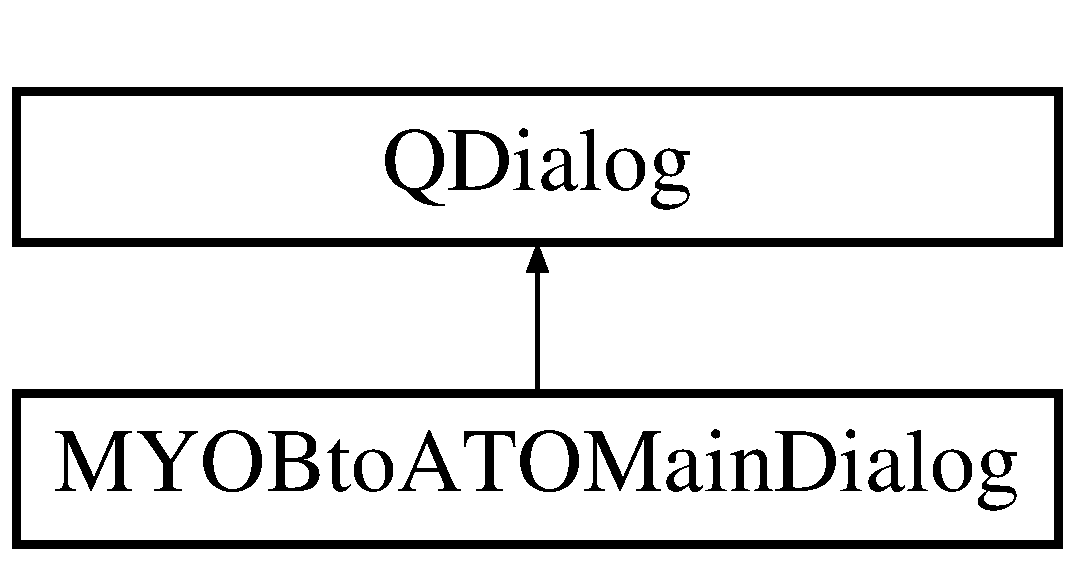
\includegraphics[height=2.000000cm]{class_m_y_o_bto_a_t_o_main_dialog}
\end{center}
\end{figure}
\subsection*{Public Member Functions}
\begin{DoxyCompactItemize}
\item 
\hypertarget{class_m_y_o_bto_a_t_o_main_dialog_a762700abdbd63aed2b7afc29bdb235a3}{}\label{class_m_y_o_bto_a_t_o_main_dialog_a762700abdbd63aed2b7afc29bdb235a3} 
{\bfseries M\+Y\+O\+Bto\+A\+T\+O\+Main\+Dialog} (Q\+Widget $\ast$parent=0)
\end{DoxyCompactItemize}


\subsection{Detailed Description}
Class creates window which opens from main window when M\+Y\+OB button clicked by user and contains buttons to open relevant files and create output 

The documentation for this class was generated from the following files\+:\begin{DoxyCompactItemize}
\item 
A\+T\+Oassignment/myobtoatomaindialog.\+h\item 
A\+T\+Oassignment/myobtoatomaindialog.\+cpp\end{DoxyCompactItemize}

%--- End generated contents ---

% Index
\backmatter
\newpage
\phantomsection
\clearemptydoublepage
\addcontentsline{toc}{chapter}{Index}
\printindex

\end{document}
